\chapter{System Design}
\label{ch:system-design}
\graphicspath{{./img/system-design/}}

This section will contain an abstracted view of the system, with blocks for antanna array, RF front end, digitisers, first stage DSP on ROACH, 2nd stage DSP on PC with ethernet link.

A brief explanation of the design considerations for each stage of the system. Stating that each block will be designed and expanded on in the following chapters.

\begin{landscape}
  \thispagestyle{empty}
  \begin{figure}
    \centering
    \makebox[\textwidth][c] {
      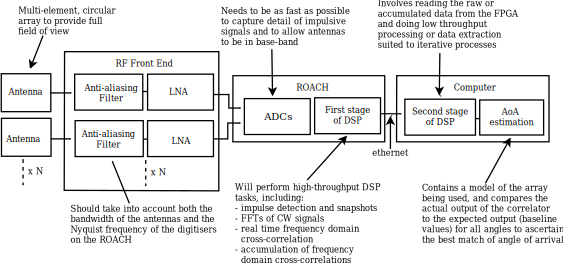
\includegraphics[width=\paperwidth, clip=true, trim = 80 500 80 80]{basic-flow}
      % left, bottom, right, top
    }
  \caption{Very abstract view of the flow of signals through the proposed DF system. The key function of the blocks has been noted on the diagram. }
  \end{figure}
\end{landscape}

\section{Direction Finding Algorithms}

Here we select what DF algorithm to use.

A simulation for the DF algorith was written in python.

The structure of the software doing the simulation is similar to the structure of the software which will be implemented.

In preperation for the implementation of the final DF algorithms, python packages were written: 
directionFinder-backend has the code for an AntennaArray class which builds an array model out Antenna objects and can the calculate and returning a vector of the antenna array manifold. The phase-ambiguity package has logic for creating an AntennaArray object and then correlating the manifold vector from a reference direction to manifold vectors from all directions to find mathces and plot the results.

Parameters:
frequency range, number of frequency points, angle range, number of angle points, reference angle.

This produces a 3-d plot. Typically the 3-d plot is flattened to a 2-D image with colour used for the third dimension, rather than rendinging a 3-d image. The type of data being plotted naturally lends itself to a colour plot view.


Ideally we would like 4 dimensional vectors: frequency, reference angle, aoa, correlation. However, this is difficult to do. Hence, two simulation strategies are used: either fix reference angle and vary frequency and aoa. Or fix frequency and vary reference and aoa. They produce results with a different view: one shows the ambiguity perforamcne and a certain frequency, the other view shows the slice of the ambiguity performance over the whole frequency range. Process:

\begin{enumerate}
  \item A configuration file specifying how an antenna array is positioned in read in an an AntennaArray object is created.
  \item For each frequency bin in the frequency range:
  \begin{enumerate}
    \item The array manifold is generated for a reference \gls{aoa}. Default: \SI{0}{\degree}.
    \item For each angle in the incident angle range:
    \begin{enumerate}
      \item Calculate manifold.
      \item Correlate.
      \item Now have data point: frequency, incident angle, correlation between reference and this.
    \end{enumerate}
  \end{enumerate}
  \item plot all data points
\end{enumerate}

How about: vary reference and aoa and then pick the worst and plot that. Or average?? What's most interesting. Worst. Let's see worst case performance. 

\section{Frequency Domain Direction Finding}
How it works. Get phase difference between visibilities. 
Discuss algorithms. 

\subsection{Ambiguity Simulations}
Various ambiguity plots. 
Also show cross section for signal at 250 MHz
\begin{figure}
  \centering
  \begin{subfigure}{\textwidth}
    \centering
    \includegraphics[width=\textwidth, clip=true, trim = 0 15 53 0]{ambiguity03}
    % left, bottom, right, top
  \end{subfigure}\\[1em]
  \begin{subfigure}{\textwidth}
    \centering
    \includegraphics[width=\textwidth, clip=true, trim = 0 15 53 0]{ambiguity04}
  \end{subfigure}\\[1em]
  \begin{subfigure}{\textwidth}
    \centering
    \includegraphics[width=\textwidth, clip=true, trim = 0 15 53 0]{ambiguity05}
  \end{subfigure}
  \caption{Ambiguity plots for various antenna array sizes with reference signal arriving at \SI{0}{\degree}.}
\end{figure}
\begin{figure}
  \ContinuedFloat
  \centering
  \begin{subfigure}{\textwidth}
    \centering
    \includegraphics[width=\textwidth, clip=true, trim = 0 15 53 0]{ambiguity06}
    % left, bottom, right, top
  \end{subfigure}\\[1em]
  \begin{subfigure}{\textwidth}
    \centering
    \includegraphics[width=\textwidth, clip=true, trim = 0 15 53 0]{ambiguity07}
  \end{subfigure}\\[1em]
  \begin{subfigure}{\textwidth}
    \centering
    \includegraphics[width=\textwidth, clip=true, trim = 0 15 53 0]{ambiguity09}
  \end{subfigure}
  \caption{(cont'd) Ambiguity plots for various antenna array sizes with reference signal arriving at \SI{0}{\degree}.}
\end{figure}

\subsection{Accuracy Simulations}
RMS phase error vs RMS angular error.
\begin{figure}
  \centering
  \includegraphics[width=0.9\textwidth]{visibility-error-vs-df-error}
  \caption{This is a graphic showing some stuff}
\end{figure}

\section{Time Domain Direction Finding}
Ambiguity not really an issue.
Discuss upsampling. Show plots.
Again, simulation:
SNR vs number of correct correlation peaks.
Table: 
For an SNR: Do 1000 different cross correlations.RMS error in number of samples.
Do SNR: 10, 5, 2, 1, 0.5, 0.2, 0.1
